\documentclass{ctexart}

\usepackage{amstext}
\usepackage{geometry}
\geometry{
  a4paper,
  total={210mm,297mm},
  left=20mm,
  right=20mm,
  top=20mm,
  bottom=20mm,
}
\usepackage{hyperref}
\hypersetup{
  bookmarksnumbered=true,
  colorlinks=true,
  allcolors=blue,
}
\usepackage[
  backend=biber,
  style=numeric,
  citestyle=ieee,
]{biblatex}
\addbibresource{translation_geometry.bib}
\usepackage{graphicx}
\usepackage{booktabs}
\usepackage{csvsimple}
\usepackage{siunitx}
\usepackage{enumerate}
\usepackage{amsmath}


\title{低矮房屋的体型对其所受龙卷风荷载影响的的研究}
\author{Jeremy Case}
\date{}

\begin{document}

\maketitle

\begin{abstract}
尽管龙卷风的破坏力巨大,但仅存在有限的尝试试图定量分析龙卷风引起的荷载。
本文的目的在于分析建筑的不同体型对其在模拟龙卷风(模拟龙卷风的涡流比根据实测龙卷风取值)作用下所受荷载和风压的影响。
测量得到的建筑所受荷载和风压被用于评估抗龙卷风设计的可行性。
龙卷风实验装置核心直径\SI{56}{m},能产生较大的涡流比(\num{2.6})以代表EF3等级龙卷风,建筑的缩尺模型放置于实验装置中,以测量其所受风压。
研究表明,最大风压与檐口高度、屋顶高度、纵横比、平面面积、及其它建筑几何形状的变化(如附加的车库、挑檐和拱腹)有关。
根据测量所得风压计算屋盖与墙、墙板与椽子的连接所需强度,并与其实际强度进行比较,以评估结构失效的概率。
结果表明,住宅中两处关键的连接(主要是屋盖与墙的连接)若设计得当,则能保证足够的安全储备以抵抗不超过EF3等级的龙卷风的袭击。
\end{abstract}

\section{引言}
许多观点质疑住宅抗龙卷风设计的可能性,遑论其可行性。
这样的观点大多来自于对结构在强风作用下的破坏程度的评估,并因龙卷风惊人的破坏力而产生偏见,
但这些观点并未依据足尺或缩尺建筑的龙卷风试验所测压力与结构构件与连接具有的实际抗力的比较。
现代工程学基于理论和经验总结的准则,但对于抗龙卷风设计,几乎没有数据能用于形成实用的工程准则。
过去,在龙卷风袭击时,屋盖所受风压及结构所受荷载的近似数据仅被用于法院的调查和工程的判断之中。
这种限制来源于三个困难:缺乏能够测量龙卷风引起的风压和荷载的仪器;缺乏实测数据与实验数据进行对比研究;
以及缺乏对抗龙卷风设计的兴趣,因为人们假定这样做是不经济的。

为了克服上文第一个困难\cite{haan2008design},爱荷华州立大学(Iowa State University, ISU)建成了一个龙卷风模拟装置。
ISU龙卷风装置能产生相对于建筑模型运动的龙卷风,也能调整多个参数以产生不同种类的龙卷风。
随着近年来几次龙卷风的实测数据的陆续发表\cite{karstens2010near}\cite{lee2005diagnosed}\cite{wurman2002multiple},第二个困难也能迎刃而解了。
随后的工作比较了ISU实验室模拟的龙卷风与实测龙卷风及计算流体力学的龙卷风模型的特征\cite{sarkar2005laboratory}。
Thampi等人的工作\cite{thampi2011finite}表明:当把低矮建筑所受ISU模拟龙卷风的风压输入到建筑的有限元模型中,相应的足尺建筑所受的破坏能够重现。
这些进步使得结构所受龙卷风荷载及风压的确定成为可能,并能据此探究经济可行的抗龙卷风设计。

本文研究了低矮建筑受到龙卷风引起的风压和荷载与建筑的几何形状及朝向的关系。
还研究了轻型木框架结构屋盖处两个最为脆弱的连接在实验室所测龙卷风风压作用下的抗掀能力,以探究抗龙卷风设计的可行性。

\section{模拟龙卷风}
只有当实验室模拟的龙卷风与实际发生的龙卷风具有相同特征时,模拟的龙卷风作用在低矮建筑上的风压才对评估抗龙卷风设计有指导意义。
为了获得结构设计所需的风压和荷载,实验室模拟的龙卷风需要具备一些关键的特征,其对结构所受荷载有着重要的影响。
根据Haan等人\cite{haan2009tornado}的研究,这些特征包括水平最大风速、龙卷风核心半径及行进轨迹、涡流比和移动速度。

\subsection{水平最大风速}
根据法院的数据,大约$90 \%$的龙卷风为F2等级或小于F2等级\cite{bluestein1993review}。
以EF(Enchanced Fujita)\cite{marshall2004enhanced}等级衡量,这对应着EF3等级的上界,据估计最大风速为\SI{74}{m/s}。
ASCE 7-10规范\cite{american1994minimum}规定美国东南部和沿海地区等级II建筑的设计风速在\SI{63}{m/s}和\SI{80}{m/s}之间,
ICC规范\cite{ibc2012international}规定相同地区的设计基本风速介于\SI{54}{m}和\SI{63}{m}。
规范规定的基本风速的范围意味着针对此风速量值进行设计是可行的。
建筑设计规范规定的设计基本风速与龙卷风的最大水平速度具有相同的量级,即\SI{74}{m/s}或更小,
选定试验模拟的龙卷风所对应的足尺龙卷风具有的水平风速为\SI{74}{m/s}。

ISU龙卷风模拟装置产生的风场在\SI{19}{mm}高度处的最大切向速度为\SI{11.6}{m/s},最大水平速度为\SI{11.7}{m/s}。
根据足尺龙卷风平均作用时间与模拟龙卷风作用时间相等的原则,
可确定最大水平风速为\SI{74}{m/s}(EF3等级)的足尺龙卷风与ISU模拟龙卷风的速度相似比为$\lambda_{\mathrm{v}}=11.7/74=1/6.3$。
根据最大切向速度归一化后的切向速度分布的等值线图见图\ref{fig:Vt-contour}。 

\begin{figure}
\centering
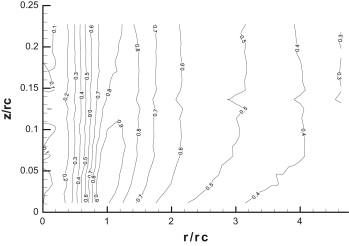
\includegraphics{./fig/1.jpg}
\caption{切向速度根据最大切向速度归一化后等值线图}
\label{fig:Vt-contour}
\end{figure}


\subsection{龙卷风核心直径}
Brooks\cite{brooks2004relationship}利用报道的龙卷风破坏路径长度和宽度的数据,将藤田级数建模成Weibull分布。
根据此分布能根据具有特定藤田等级龙卷风出现的发生概率,计算其破坏路径宽度的概率。
这项研究表明,龙卷风的平均破坏宽度随藤田等级的提高而增大。
根据Brooks的结果\cite{brooks2004relationship},F1或F2等级(近似等同于EF2和EF3等级)的龙卷风,其其路径宽度近似介于\SI{100}{m}和\SI{500}{m}之间。

假定当风速达到规范规定的风速时,建筑出现破坏,对于美国中西部,设计基本风速为\SI{40}{m/s},
而EF3等级龙卷风的最大水平速度为\SI{74}{m/s},建筑的破坏可能发生在一定的范围内,这一范围可由水平风速近似超过最大切向速度的一半确定。
图\ref{fig:Vt-contour}中0.5等值线位于地表高度处大概2.2倍最大风速半径(核心半径)处。
根据Brooks的研究,EF3等级龙卷风的核心半径有很大的概率介于\SI{45}{m}和\SI{225}{m}之间。
本文的模拟龙卷风的核心半径为\SI{0.56}{m},当根据长度相似比$1:100$进行放大后,与Brooks研究得到的核心半径相符。

\subsection{涡流比}
实验室模拟龙卷风和数值模拟龙卷风最常用的参数之一是涡流比\cite{haan2008design} \cite{hangan2008swirl}。
涡流比($S$)定义为切向动量与hexin核心半径处流量($Q$)的比值,
即$S=\pi V_{\theta \mathrm{max}}r_c^2/Q$,其中$r_c$是核心半径,
$r_c$处的切向速度为最大切向速度$V_{\theta \mathrm{max}}$。
多项研究都表明涡流比是决定龙卷风风场特征的参数\cite{hangan2008swirl}\cite{church1979characteristics}\cite{davies1973dependence}。
Davies Jones展示,核心半径是涡流比的函数。
Davies Jones和Church发现涡旋的结构与涡流比相关:当涡流比增大时,涡旋分裂成多个涡旋\cite{davies1973dependence}。

足尺龙卷风的数据显示,涡流比为\num{2.0}或更大。
例如,Hangan和Kim通过比较Spencer, South Dakota发生的龙卷风与3D数值模拟龙卷风\cite{hangan2008swirl},发现涡流比最合适的设定为$S=2.0$。
根据车载多普勒雷达(DOW)测得的数据,Lee和Wurman等人\cite{lee2005diagnosed}计算得到,Mulhall龙卷风的涡流比介于\num{2}和\num{6}之间。
这些涡流比都是根据涡旋核心半径处($r_c$)的数据计算得到。
根据DOW测得的最新数据,并与数值模拟结果进行对比,可以发现涡流比应该增大至\num{2}或更大。
ISU龙卷风模拟装置中,产生上升气流的风口的直径为\SI{1.8}{\meter}。
气流随后直接被同心的管道引导成下降的气流。
旋转的气流通过与管道径向成一定角度的固定叶片产生。
ISU龙卷风装置可通过增大叶片角度\cite{haan2008design}以提高涡流比。
为了获得较大的涡流比,叶片的角度设置成\SI{75}{\degree},得到的核心半径处的涡流比为\num{2.6}。

\subsection{移动速度}
据报道,实际发生的龙卷风具有不同的移动速度:\SI{16.5}{m/s}\cite{thampi2011finite},\SI{13}{m/s}\cite{lee2005diagnosed}和\SI{23}{m/s}\cite{haan2008design}。
根据这些报道,实验室测量移动速度为\SI{0.15}{m/s}的龙卷风作用在建筑上的风压。
如果假定建筑所受破坏与其受龙卷风袭击的时间成正比,则涡旋的移动时间的相似比($\lambda_T$)应该等于$1$。
这样的设置保证了涡旋平移速度的相似比与长度的相似比一致。
因此,龙卷风装置的平移速度 \SI{1.15}{m/s}考虑到长度相似比($\lambda_L=1:100$)后,对应的足尺龙卷风的移动速度为\SI{15}{m/s}。

\subsection{地面粗糙度}
本试验用涂了清漆的胶合板模拟地面,这种胶合板很光滑。
没有引起地面粗糙的突起存在,因此可以模拟开阔平整的地面。
因为大部分的“龙卷风走廊”是乡间的农田,开阔平整的地面是合理有效的模拟对象。

\section{建筑模型,量测仪器,数据处理}
\subsection{建筑模型}
分别测量9种坡屋盖建筑模型的风压(图\ref{fig:building-models}):
不同的屋面倾角(\num{4.6}-\SI{35.5}{\degree}),屋脊高度(\num{12.2}-\SI{36}{ft}),
$L/B$比值(\num{1.0}和\num{1.5};其中$L$是长度,$B$是宽度)和
$h/L$比值(\num{0.34}-\num{0.8};其中$h$是平均屋盖高度),
是否有附属车库,并且设置多种试验工况以考虑建筑模型相对于龙卷风行进轨迹的方位角的影响。
% pressure taps
每个模型都贴有最多\num{124}个压强贴。

\begin{figure}
\centering
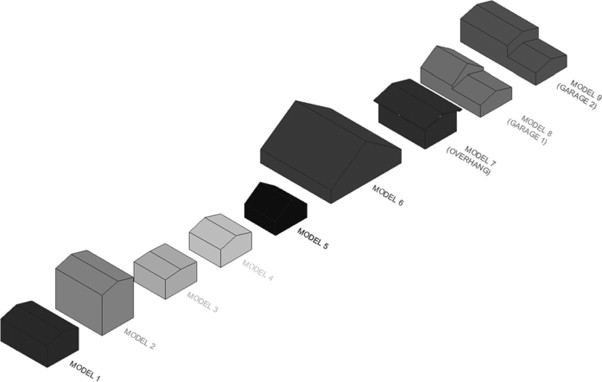
\includegraphics{./fig/2}
\caption{研究所用建筑模型}
\label{fig:building-models}
\end{figure}


模型的几何尺寸根据实际建筑尺寸经过$1:100$的相似比放大后确定,
这样才能根据试验中建筑模型的屋盖高度、纵横比、屋面倾角、挑檐距离和附加车库对模型所受模拟龙卷风的风压和荷载的影响,推测实际的情况。
模型尺寸根据常规的简易房屋设计确定,并参考ASCE 7-10规范中图6-6\cite{american1994minimum}确定,该图将风压系数列成平均屋盖高度与建筑长度、风向和屋面倾角的比值间关系的表格。
模型尺寸列于表\ref{tab:1}。

\begin{table}\label{tab:1}
\csvautobooktabular{./tab/table.csv}
\end{table}


\subsection{量测仪器}
对于静止龙卷风,采用Cobra探头(多孔探头,TFI\textregistered )测量风速,采样频率为\SI{78.1}{Hz},采样时间为\SI{26}{s}。
测点的布置间距水平向为\SI{50.8}{mm},竖向为\SI{6.35}{mm}。
测点竖向从\SI{6.35}{mm}处开始布置,直到高度为\SI{127}{mm},每竖向高度处水平布置长度为\SI{2.54}{m}。

采用两个高速64频道ZOC33/64Px压强传感器(Scanivalve Corporation\textregistered ),以\SI{390}{Hz}的采样频率测量风压。
在风压和风速量测中,仪器静压设置为实验室大气压。

\subsection{试验步骤和数据处理}
对每种工况,共测量10次风压。
对10次试验量测的风压峰值进行简单平均,作为峰值风压。
建筑模型相对于龙卷风行进路径的角度(Building Orientation Angle,BOA)(图\ref{fig:BOA})从\SI{0}{\degree}变化到\SI{90}{\degree},角度步长为\SI{15}{\degree}。
BOA为\SI{0}{\degree}对应着龙卷风行进方向与建筑模型的屋脊平行(沿着长度 $L$方向)。
车库模型的设置角度从\SI{0}{\degree}到\SI{90}{\degree}(方位1)和\SI{180}{\degree}到\SI{270}{\degree}(方位2)。
在方位1的情况,较高的车库模型先经历龙卷风,方位2时,较低的车库模型先经历龙卷风。
所有试验工况,龙卷风的行进路径都经过建筑模型的中心。

\begin{figure}
\centering
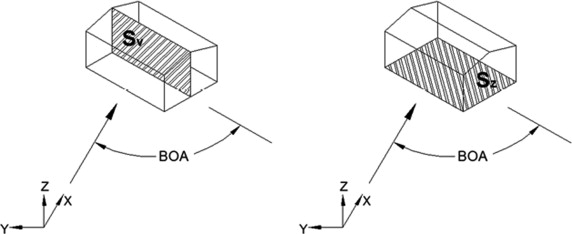
\includegraphics{./fig/3}
\caption{建筑模型相对于龙卷风行进方向轴($X$)的方位角(BOA)及用于风压系数归一化的面积($S_v$, $S_z$)}
\label{fig:BOA}
\end{figure}


风压系数沿如下方向计算:$x$向(平行于龙卷风行进方向的水平方向);$y$向(垂直于龙卷风行进方向的水平方向);$z$向(竖向)。
平面$xy$上的风ya压系数 ($C_{Fxy}$)为$x$向风压系数($C_{Fx}$)和$y$向风压系数($C_{Fy}$)平方和的根,是一个表征低矮建筑所受风荷载的重要参数。
$x$向和$y$向的风压系数利用面积$S_v$进行归一化,其中$S_v$等于屋脊高度与屋脊长度的乘积。
$z$向的风压系数利用面积$S_z$进行归一化,其中$S_z$等于建筑平面面积。
上述归一化风压系数的公式可表示为:
\begin{equation}
	C_{Fx}=\frac{F_x}{(1/2)\rho V_H^2 S_v}
\end{equation}

\begin{equation}
	C_{Fy}=\frac{F_y}{(1/2)\rho V_H^2 S_v}
\end{equation}

\begin{equation}
	C_{Fx}=\frac{F_z}{(1/2)\rho V_H^2 S_z}
\end{equation}

\begin{equation}
	C_{Fxy}=\sqrt{C_{Fx}^2+C_{Fy}^2}
\end{equation}

\section{结论}
对每个模型在每一建筑方位角的工况,计算其峰值风压和风压系数及其时程,并绘图表示。
通过比较不同模型的峰值风压和风压系数及其时程,展示不同体型的影响。
描述体型的变量中只有一个不同的模型相互比较,以隔离这一变量的影响。

\subsection{屋脊高度}
模型1和模型2具有相同的平面面积和平面纵横比。两个模型的不同之处在于屋脊高度:模型2的屋脊高度(\SI{110}{mm})几乎是模型1(\SI{60}{mm})的两倍。
对任一建筑方位角(BOA),两个模型的峰值风压的等值线图是相似的,但幅值不同。
模型1的峰值风压明显更大。
两个模型的屋脊高度均比测量最大切向速度处的高度(\SI{19.5}{mm})要大。
模型1屋脊高度处的最大切向速度为\SI{10.6}{m/s},模型2屋脊高度处的最大切向速度为\SI{9.6}{m/s}。
这说明了峰值风压与屋脊高度有关。
模型1和2在建筑方位角为\SI{30}{\degree}时的平均峰值风压的等值线图见图\ref{fig:ppc}。
模型1和2在方位角为\SI{30}{\degree}时的风压系数$C_{Fz}$和$C_{Fxy}$的时程曲线见图\ref{fig:Cfz}和\ref{fig:Cfxy}。
\begin{figure}[h]
\centering
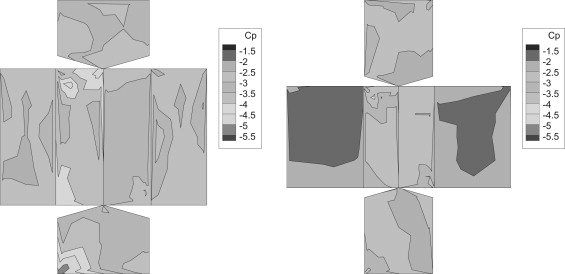
\includegraphics{./fig/4.jpg}
\caption{模型1(左)和模型2(右)在方位角为\SI{30}{\degree}时的风压等值线图}
\label{fig:ppc}
\end{figure}

\begin{figure}[h]
\centering
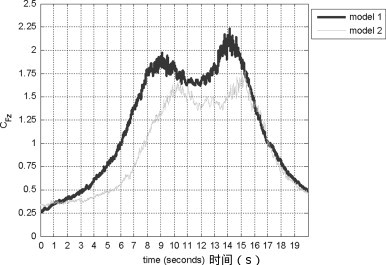
\includegraphics{./fig/5.jpg}
\caption{模型1和2在BOA为\SI{30}{\degree}时的竖向风压系数时程图}
\label{fig:Cfz}
\end{figure}

\begin{figure}[h]
\centering
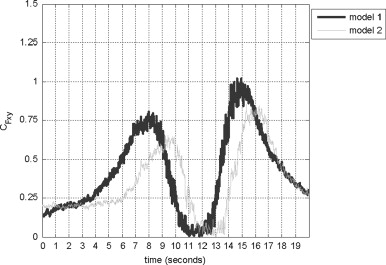
\includegraphics{./fig/6.jpg}
\caption{模型1和2在BOA为\SI{30}{\degree}时的$XY$向风压系数时程图}
\label{fig:Cfxy}
\end{figure}

\subsection{屋面倾角的影响}
比较模型3、4和5以探究屋面倾角对龙卷风引起的风压和荷载的影响。
三个模型具有相同的屋面平均高度(\SI{55}{mm}),相同的平面尺寸,以及相同的纵横比($L/B=1.0$,$h/L=0.56$)。
模型3的屋面倾角是\SI{4.6}{\degree},模型4的屋面倾角是\SI{15.95}{\degree},模型6的屋面倾角为\SI{35.5}{\degree}。
平均风压峰值有明显的变化趋势:当屋面倾角增大时,屋面的风压峰值的幅值减小,而墙的风压峰值增大。
对于模型3和4,峰值风压$C_{Fz}$出现在建筑方位角为\SI{45}{\degree}时,对于模型5,峰值风压 $C_{Fz}$出现在建筑方位角为\SI{60}{\degree}时。
建筑方位角为\SI{45}{\degree}时,模型3、4和5的平均峰值风压等值线图见\ref{fig:p-pitch}。
\begin{figure}[h]
\centering
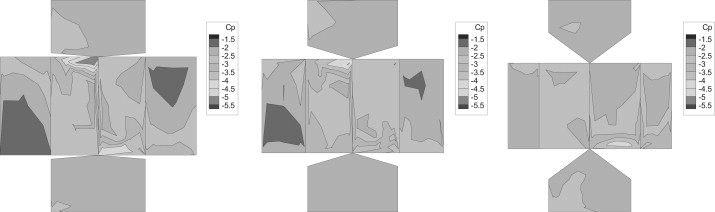
\includegraphics{./fig/7.jpg}
\caption{模型3(左)、4(中)、5(右)在BOA为\SI{45}{\degree}时的峰值风压等值线图}
\label{fig:p-pitch}
\end{figure}

Haan等\cite{haan2009tornado}发现,龙卷风引起的峰值上吸力不随建筑方位角变化。
图\ref{fig:uplift}验证了这一发现,也展示了峰值上吸力也不随模型3、4和5的屋面倾角而变化。
峰值风压会随屋面倾角变化,但风压系数并不明显随之变化,因为峰值风压并不一定同时出现在所有位置,而风压分布的积分产生了最大的风压系数。
\begin{figure}[h]
\centering
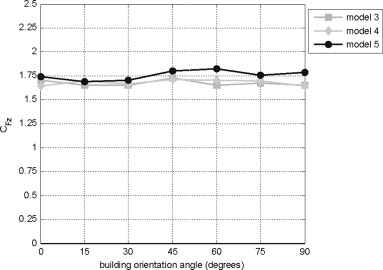
\includegraphics{./fig/8.jpg}
\caption{模型3、4和5在不同方位角的峰值风压系数}
\label{fig:uplift}
\end{figure}

\subsection{平面尺寸的影响}
与模型1在屋脊高度处的最大切向速度相比,模型2屋脊处较小的最大切向速度可能引起了峰值风压和竖向风压系数与模型1的不同。
模型4与模型1和2具有相同的屋面倾角,但屋脊高度为\SI{48}{mm}。
该高度处的最大切向速度为\SI{10.85}{m/s},比模型1(\SI{10.6}{m/s})和模型2(\SI{9.6}{m/s})都要高,但模型1的峰值$C_{Fz}$仍比模型4大。
模型4和模型1的最大的不同之处在于比值$L/B$,成为建筑的纵横比。
模型1的纵横比为\num{1.5},而模型4的纵横比只有\num{1.0}。
通过比较模型4由龙卷风引起的风压系数$C_{Fz}$的时程曲线图\ref{fig:9}和模型1和2的时程曲线图\ref{fig:Cfz},可以看出纵横比的重要影响。
模型1和2的风压系数$C_{Fz}$的时程曲线中,初始峰值后出现一段较低的风压系数值,然后又出现另一个风压系数峰值(当龙卷风即将离开建筑时)。
这与模型4的$C_{Fz}$的时程曲线不同:模型4的$C_{Fz}$的时程曲线在龙卷风经过建筑的过程中基本保持恒定。
当纵横比大于1时,切向速度对于增大所有模型的峰值$C_{Fz}$系数才有重大影响。

比较图\ref{fig:Cfz}中模型1和图\ref{fig:13}中模型6的$C_{Fz}$时程,可以发现$C_{Fz}$的时程曲线的不同形状是由于建筑平面的纵横比,并非建筑的总长。
虽然模型6的总长为\SI{221}{mm},而模型1的总长只有\SI{146}{mm},但模型6的时程曲线与其他纵横比为\num{1.0}的模型的时程曲线的形状是相似的。
\begin{figure}
\centering
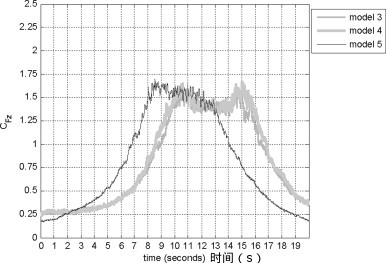
\includegraphics[width=0.7\linewidth]{./fig/9.jpg}
\caption{模型3、4和5在建筑方位角为\SI{30}{\degree}时的$C_{Fz}$时程曲线}
\label{fig:9}
\end{figure}

\subsection{挑檐和拱腹的影响}
对于低矮建筑,研究挑檐和拱腹对龙卷风荷载的影响具有重要意义,因为美国的低矮建筑一半都有挑檐和封闭的拱腹。
除了设置有挑檐和拱腹的模型7(下文称为挑檐模型),其它所有模型在屋盖与墙相交处都是尖角。
挑檐模型完全类似于模型1,除了挑檐和拱腹部分。
所有模型均不考虑内部压强。

测量拱腹下部的风压。
拱腹下部的峰值风压介于\num{1.0}到\num{3.0}之间,与建筑方位角和拱腹区域相关。
虽然拱腹处峰值风压的量值远小于模型1,但二者的风压等值线的形状是类似的。
另外,拱腹对墙面峰值风压的分布影响较屋面峰值风压的影响小。
图\ref{fig:10}显示了模型1和挑檐模型在建筑方位角为\SI{30}{\degree}时的峰值风压等值线图。
\begin{figure}
\centering
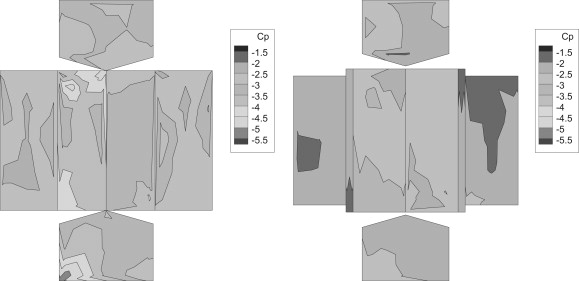
\includegraphics[width=0.7\linewidth]{./fig/10.jpg}
\caption{模型1(左)和挑檐模型(右)在\SI{30}{\degree}方位角时的峰值风压分布}
\label{fig:10}
\end{figure}

图\ref{fig:11}显示了增设挑檐对竖向风压系数的重要影响。
类似于峰值风压,水平风压系数受到挑檐的影响要小于竖向风压系数。
这可以从图\ref{fig:12}中看出。
\begin{figure}
\centering
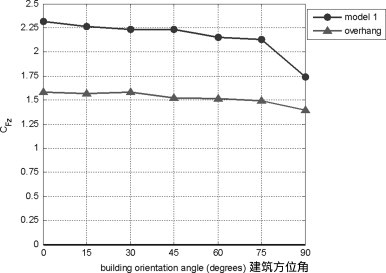
\includegraphics{./fig/11.jpg}
\caption{模型1和挑檐模型7在各建筑方位角时的峰值竖向风压系数}
\label{fig:11}
\end{figure}

\begin{figure}
\centering
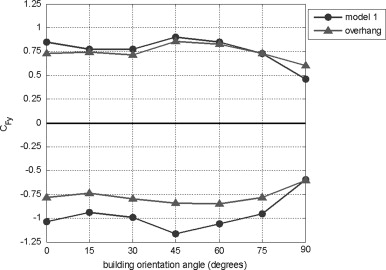
\includegraphics{./fig/12.jpg}
\caption{模型1和挑檐模型7在各建筑方位角时的峰值水平风压系数}
\label{fig:12}
\end{figure}

\subsection{平面面积和高宽比的影响}
模型5和模型6的屋面倾角($\theta$)均为\SI{35.5}{\degree},屋脊高度($h_e$)均为\SI{37}{mm},
纵横比($L/B$)均为\num{1.0},但有不同的平面尺寸,分别为\SI{98}{mm}和\SI{221}{mm},
以及不同的总高度($h_t$),分别是\SI{72}{mm}和\SI{114}{mm}。
由这些尺寸可以计算模型5和模型6的平均屋盖高度和长度的比值($h/L$)。
模型6的尺寸比模型5的较大,来产生不同的$h/L$的数值。
其平面尺寸几乎是龙卷风核心半径的$40\%$。
这导致了建筑结构必须承担更长时间的 龙卷风荷载,如图\ref{fig:13}所示。
\begin{figure}
\centering
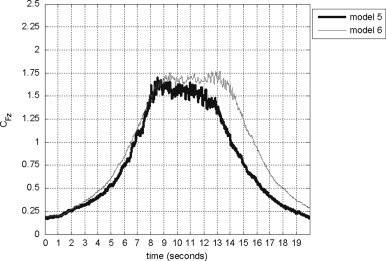
\includegraphics{./fig/13.jpg}
\caption{模型5和模型6在\SI{30}{\degree}方位角时的竖向风压系数时程曲线}
\label{fig:13}
\end{figure}

\subsection{附加车库的影响}
美国的大多数民用住宅都附有车库。
附加车库的高度一般比主体住宅低,二者具有平行的屋脊。
本试验测试了两个附有车库的模型。
模型8或车库模型1带有附加车库,除此之外,与模型5完全一样。
类似的,模型9或车库模型2是模型2的复制,除了模型9带有附加车库。
两个模型的车库的尺寸、屋脊高度和屋面倾角是完全一致的。
类似于其他模型,车库模型的建筑方位角从\SI{0}{\degree}以\SI{15}{\degree}的步长变换,并测量并记录风压。
对每个车库模型,这一步骤都操作两次:一次模拟龙卷风先袭击模型主体建筑(方位1);一次模拟龙卷风先袭击车库部分(方位2)。

附加的车库增大了原始模型的纵横比($L/B$)。
纵横比的增大引起了车库模型1比模型5(不带车库)在多数建筑方位角时具有更大的峰值竖向风压系数。
然而对于车库模型2,峰值竖向风压系数比纵横比($L/B$)的模型更大,却在多数建筑方位角的情况下比模型1较小。

附加车库引起了更为复杂的几何形状,导致建筑模型与龙卷风之间的相互作用变得更为复杂。
对这种相互作用的研究需要测试更多的模型以完全理解附加车库的影响。

\subsection{建筑体型对屋盖连接所需承载力的影响}
通过比较$X$、$Y$和$Z$向峰值风压系数,可以发现在每个建筑方位角的情况,竖向风压系数总是大于两个方向的水平风压系数,有时其比例达到了\num{2}。
对所有模型,峰值风压系数出现在屋面上。
屋面所受峰值风压和风压系数均为负,沿屋面向外作用,引起屋盖连接受到向上的吸力。
着与Haan\cite{haan2009tornado}的发现相符。

据此不难理解龙卷风发生后调查报告指出的大多数民用住宅的破坏是由于屋盖的破坏。
而下述事实加重了屋盖破坏的情况:即在龙卷风经常发生的地区,民用住宅的屋盖到墙进而到基础的荷载传递路线上,连接几乎总是栓钉连接。
栓钉连接提高了屋盖在吸力作用下的破坏的可能性,因为栓钉连接在受拉方向承载力很低。
屋盖的破坏提高了住宅其余部位的破坏风险,因为外墙是由膜片拼合而成,并在屋盖处用交叉的支撑固定\cite{marshall2002tornado}。
因此,屋盖对住宅抗龙卷风起着重要作用。
另外,连接是屋盖在龙卷风荷载传递路径上的薄弱点,因此提高住宅抗龙卷风能力的关键在于加强这些连接。

Sparks等人\cite{sparks1988failure}指出低矮房屋的屋盖对结构整体性起着重要作用,对于直线型风,屋盖连接不仅与风速而且与屋盖几何形状有关。
这些研究者也发现,整个住宅会在屋盖破坏后迅速失效。
根据这些研究成果,可以推知屋盖桁架和立柱墙之间的连接对于整个住宅体系能否经受龙卷风的重要意义\cite{sparks1988failure}。
除了屋盖与墙连接(RTWC)的重要性之外,他们也发现:对于几种不同的屋盖几何形状,栓钉RTWC会在风速小于\SI{54}{mph}时失效,这比边界层风速\SI{90}{mph}小的多。

低矮民用住宅的破坏的顺序一直没能被很好理解。
Thampi等人\cite{thampi2011finite}发现一旦维护结构由于风压或风致碎片发生破坏,内部的压力会改变结构失效的顺序及失效的状态。
Thampi等人\cite{thampi2011finite}还指出,密闭房屋的破坏是由于屋盖的破坏,而门的破坏引起了山墙的破坏。
因此,为了研究结构抗龙卷风设计,理解最初的破坏发生在何处具有重要意义。
由于低矮房屋在龙卷风作用下破坏顺序的复杂性,下文对屋盖连接的分析假定:在屋盖连接破坏前,结构的其余部分保持完好。

模型1和模型5用于比较屋盖连接承受的由龙卷风引起的荷载与文献中提出的屋盖连接具有的承载能力,并且分析几何尺寸和屋面倾角对连接所承担荷载的影响。
首先,利用公式\eqref{eqn:Cp}将两个模型的风压时程转化为风压系数时程,式中$P_i$是时间步$i$时记录的风压(总风压减静压),$V_H$为核心半径处平均水平风速分量,$\rho$是空气的密度。
\begin{equation} \label{eqn:Cp}
C_p=\frac{P_i}{(1/2) \rho V_H^2}
\end{equation}

\subsection{屋盖墙板连接}
空气动力学领域中,常用术语“迎风向”、“背风向”、“前缘”、“后缘”等代指淹没于直线型流场中物体的某一部分。
在龙卷风流场中,这些术语较难定义,但是考虑到缺乏可以代替的术语,下文的讨论仍沿袭这些术语。
如下的术语用于定义当建筑方位角为\SI{0}{\degree}、涡旋为逆时针旋转时,流场中物体的各个侧面。
由这些术语定义的侧面并不随建筑方位角而变化。
这些术语定义如下:

\begin{itemize}
\item 迎风向:先经历切向速度分量并且平行于龙卷风移动方向的侧面。
\item 背风向:平行于迎风向侧面的侧面。
\item 前缘:与龙卷风移动方向垂直的侧面,且在龙卷风袭击模型前离其最近的侧面。
\item 后缘:与龙卷风移动方向垂直的侧面,且在龙卷风袭击模型后离其最近的侧面。
\end{itemize}

当建筑方位角为\SI{0}{\degree}时,模型1的峰值风压出现在前缘、背风面角部和屋盖边缘。
当建筑方位角介于\SI{15}{\degree}和\SI{75}{\degree}之间时,模型1的峰值风压出现在后缘背风向屋盖边缘和迎风向前缘屋盖边缘处,
而对于模型5,峰值风压主要出现在前缘迎风向屋盖边缘和迎风向前缘处墙的边缘。
当建筑方位角为\SI{90}{\degree}时,建筑的峰值风压比建筑方位角取其它值时小,
此时模型1的峰值风压出现于屋盖的后缘迎风向区域,模型5的峰值风压出现于屋盖的前缘背风向区域。
对于建筑方位角取所有值的情况,模型1的最大峰值风压系数为\num{6.1},模型5的为\num{4.9}。

根据模型1和模型5的最大峰值风压系数和采用不同栓钉连接形式的承载能力,计算能引起屋盖连接发生破坏的临界风速。
不同栓钉类型和栓钉间距的连接,发生破坏的临界龙卷风水平风速列于表\ref{tab:2},
表中风速对应足尺龙卷风,根据与模拟龙卷风作用相同时间的准则确定。
以较小间距安装8d圆形柄栓钉代替6d光滑柄栓钉,增加的费用与住宅全部费用相比较少。
而如果这一设置减少了因龙卷风造成的损失,则微小的费用增加是合理的。


\subsection{屋盖与墙的连接}
为了获得足尺屋盖和墙连接的反应,模拟龙卷风的最大水平速度放大到足尺龙卷风风速\SI{74}{m/s},
根据模拟龙卷风与足尺龙卷风平均作用时间相同。
根据速度相似比($1:15.9$)和长度相似比($1:6.3$)可以计算出时间相似比$\lambda_T$为$1:59$。

将模型尺寸根据长度相似比$\lambda_L=1:100$放大称实际尺寸。
实际住宅屋盖桁架的间距为\SI{0.6}{m}。
对于这些特定模型,无法获取其影响函数,故采用矩形的附属面积。
各个格点处区块(图\ref{fig:14})对应于某一桁架和压强贴。
利用风压系数时程和式\ref{eqn:Cp},计算足尺龙卷风作用下每一时间步每处区块的风压。
分析假定各区块上风压是均匀分布的。

\begin{figure}
\centering
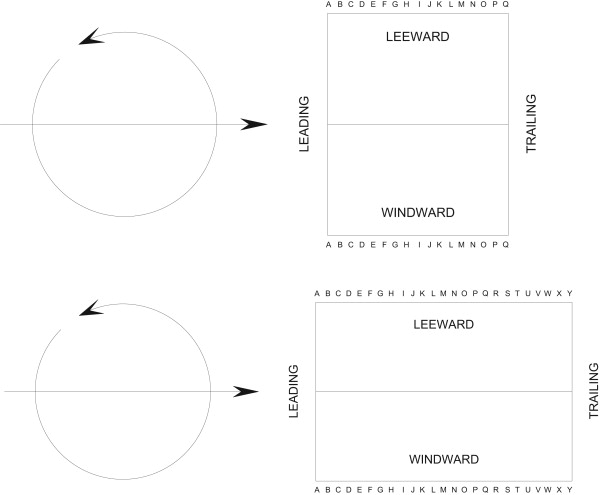
\includegraphics{./fig/14.jpg}
\caption{模型1(上)和模型5(下)桁架连接相对于龙卷风的位置}
\label{fig:14}
\end{figure}


计算得到每一区块上作用的风荷载,及其竖向分量与恒载作用下桁架和连接处内力的差值,
以确定龙卷风作用下桁架的内力(图\ref{fig:15}和\ref{fig:16})。

\begin{figure}
\centering
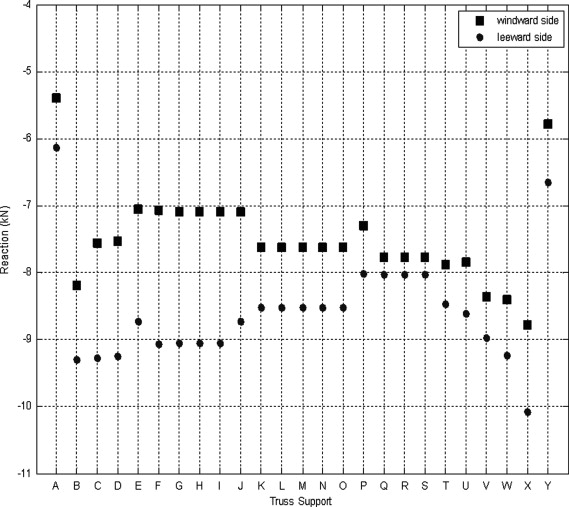
\includegraphics{./fig/15.jpg}
\caption{模型1的峰值屋盖桁架内力}
\label{fig:15}
\end{figure}

\begin{figure}
\centering
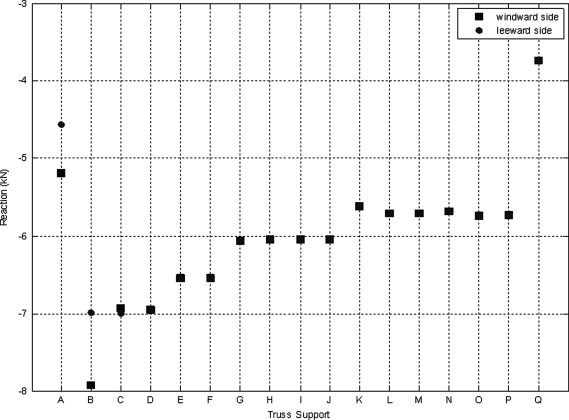
\includegraphics{./fig/16.jpg}
\caption{模型5的峰值屋盖桁架内力}
\label{fig:16}
\end{figure}



模型1的背风向比迎风向出现了较大的内力。
最大值出现于图\ref{fig:14}中背风向桁架X的竖向反力分量。
两个模型的峰值反力均为\SI{10}{kN}。
这几乎是常见的18型飓风带承载能力的2倍\cite{canfield1991uplift},是16d型栓钉连接的5倍。
这明显意味着栓钉连接是不足够的,需要通过飓风带的应用以显著提升其承载能力。
一种能提高TRWC承载能力的方法是同时使用栓钉连接和飓风带连接。
Reed等\cite{reed1997uplift}发现栓钉和飓风带的协同作用提高了RTWC的承载能力。

Cranfield等\cite{canfield1991uplift}发现,大多数飓风带的破坏是由于飓风带金属部分的撕裂。
因此,另一个解决方法是采用16型甚至14型飓风带。

上述的飓风带在美国的五金店均有出售,价钱为每条US\$0.60。
额外增加两条飓风带的花费与整个住宅的建设费用相比是微不足道的。 	

\printbibliography

\end{document}
